\documentclass{article}
\usepackage[T1]{fontenc}
\usepackage{lmodern}
\usepackage{graphicx}
\usepackage{amsmath,amssymb}
\usepackage[a4paper,margin=2cm]{geometry}
\usepackage[absolute,overlay]{textpos}
\setlength{\TPHorizModule}{1mm}
\setlength{\TPVertModule}{1mm}
\usepackage[indonesian]{babel}
\usepackage{hyperref}
\setlength{\emergencystretch}{2em}
% unit: Halaman 38

\begin{document}

% === Halaman 38 (python/native) ===

Steganography has its place in security. It is not 

intended to replace cryptography but 

supplement it. Hiding a message with 

steganography methods reduces the chance of a 

message being detected. However, if that 

message is also encrypted, if discovered, it must 

also be cracked (yet another layer of protection). 

 (David Kahn, penulis buku The Codebreakers - 

The Story of Secret Writing )

38

% deskripsi: gambar native xref 194
\noindent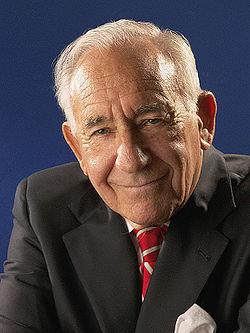
\includegraphics[width=0.85\textwidth]{../../images/python/page_038_img_01.jpeg}

\end{document}
